\chapter{Implementacja i działanie systemu Team Challenge}

\section{Środowisko implementacji}

Implementacja systemu odbywała się przy użyciu komputera wyposażonego w 8GB pamięci fizycznej oraz cztero-rdzeniowy procesor Intel Core i5-6300HQ (taktowanie 2.30GHz). Sprzęt o przytoczonych parametrach okazał się w pełni wystarczający dla przebiegu implementacji oraz lokalnego uruchamiania serwera aplikacji. Systemem operacyjnym używanym przy implementacji był Windows w wersji 10 Education. Wszystkie użyte programy i narzędzia dobrze współpracują z tym systemem.

\subsection{Wykorzystane narzędzia}


\begin{table}[H]
\centering\small
\caption{Zestawienie narzędzi wykorzystywanych podczas implementacji systemu}
\label{tab:szablon}
\begin{tabularx}{\linewidth}{|p{.2\linewidth}|p{.1\linewidth}|p{.1\linewidth}|X|}\hline
Nazwa programu & Wersja & Producent & Cel\\ \hline\hline

IntelliJ IDEA & 2018.2 & Jetbrains & Implementacja aplikacji serwerowej (Java) \\ \hline

Webstorm & 2018.2 & Jetbrains & Implementacja aplikacji klienckiej (Angular) \\ \hline

Postman & 6.5.2 & Postman & Testowanie końcówek RESTowych aplikacji serwerowej \\ \hline

Google Chrome & 70 & Google & Testowanie aplikacji klienckiej \\ \hline

Git & 2.18.0 & - & Kontrola wersji \\ \hline

\end{tabularx}
\end{table}

\section{Implementacja aplikacji serwerowej}

\subsection{Struktura projektu}

Podstawowy szkielet projektu został utworzony przy użyciu Spring Initializr. Jako narzędzie służące do zarządzania zależnościami oraz budowy projektu wybrany został Apache Maven. 

\begin{comment}
W tabeli zostały przedstawione wykorzystane moduły Springa oraz inne biblioteki. 
\end{comment}

  Klasy tworzące aplikację serwerową zostały podzielone na pakiety pod względem tematycznym, co zaprezentowano na rysunku~\ref{fig:packages}. Podział taki pozwala na utrzymanie płaskiej struktury katalogów, a w związku z tym umożliwia szybkie odnajdywanie pożądanych plików.
  
  
\begin{figure}[ht]
\centering
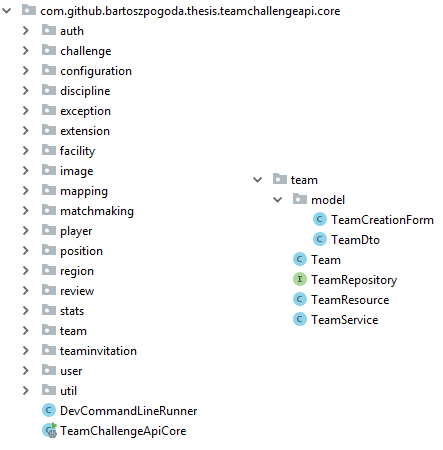
\includegraphics[width=0.5\linewidth]{06-implementacja/rys/package-team.PNG}
\caption{Fragment struktury pakietów}
\label{fig:packages}
\end{figure}

\subsection{Architektura wielowarstwowa}

Podczas projektowania architektury aplikacji ważne jest aby była ona przejrzysta oraz otwarta na rozszerzanie. Jedną z cech, którą powinny posiadać komponenty dobrze zaprojektowanego oprogramowania zorientowanego obiektowo jest ograniczenie odpowiedzialności. Jedną z metod rozdzielania odpowiedzialności jest wyszczególnienie w projekcie warstw komponentów. Aplikacja serwerowa będąca przedmiotem niniejszej pracy została podzielona na warstwy zgodnie ze standardami zdefiniowanymi dla szkieletu Spring. Wyszczególnione warstwy wraz z kierunkami komunikacji zostały przedstawione na rysunku~\ref{fig:app-layers}.


\begin{comment}

Nawiazanie do: 
Understanding Spring Web Application Architecture: The Classic Way
Petri Kainulainen October 19, 2014
https://www.petrikainulainen.net/software-development/design/understanding-spring-web-application-architecture-the-classic-way/

\end{comment}

\begin{figure}[H]
\centering
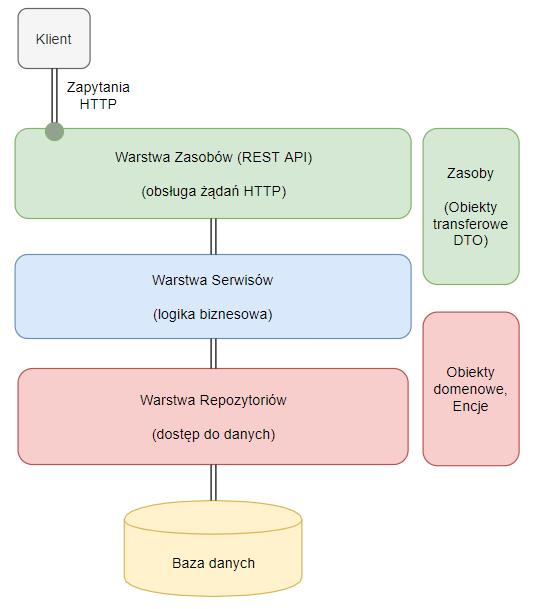
\includegraphics[width=0.5\linewidth]{06-implementacja/rys/layers.PNG}
\caption{Warstwy aplikacji serwerowej}
\label{fig:app-layers}
\end{figure}


\subsection{Warstwa repozytoriów}

Repozytoria w frameworku Spring stanowią mechanizm dostępu do danych. Warstwa ta jest abstrakcją ukrywającą przed programistą szczegóły komunikacji z bazą danych takie jak: nawiązywanie oraz utrzymywanie połączenia, konstrukcja i wykonywanie zapytań, mapowanie wyników. Deklaracja fizycznych powiązań między aplikacją a bazą danych odbywa się za pomocą adnotacji. Na listingu~\ref{list:entity} przedstawiono powiązanie encji Team z fizyczną tabelą o nazwie Teams oraz mapowania przykładowych kolumn.

\begin{lstlisting}[label=list:entity, caption=Fragment przykładowej encji, basicstyle=\footnotesize\ttfamily]
@Entity
@Table(name = "Teams")
@Data
@Builder
public class Team {

    @Id
    @GeneratedValue(strategy = GenerationType.IDENTITY)
    @Column(name = "TeamID")
    private String id;

    @OneToOne(fetch = FetchType.EAGER)
    @JoinColumn(name = "ManagerID")
    private Player manager;

    @OneToMany(mappedBy = "team", cascade = CascadeType.ALL)
    private List<Player> players;
    
    // other fields with their mappings...
}
\end{lstlisting}

Dostęp do danych zapewniają repozytoria, czyli interfejsy oznaczone adnotacją @Repository. Wygodne jest rozszerzanie dostarczonego przez moduł Spring Data interfejsu CrudRepository, który definiuje podstawowe metody dostępu takie jak dodawanie, czytanie, modyfikacja oraz usuwanie encji. Pozostałe metody potrzebne do realizacji logiki biznesowej można definiować poprzez tworzenie metod o nazwach specyfikujących ich działanie. Fizyczne zapytania do bazy danych wyznaczane są na podstawie nazwy metody. Przykładową definicję repozytorium przedstawiono na listingu~\ref{list:repository}.

\begin{lstlisting}[label=list:repository, caption=Definicja przykładowego repozytorium, basicstyle=\footnotesize\ttfamily]
@Repository
public interface TeamRepository 
extends CrudRepository<Team, String>, JpaSpecificationExecutor<Team> {

    Optional<Team> findById(String id);

    List<Team> findByRegionIdAndDisciplineIdAndActiveIsTrue(String regionId,
     String disciplineId);
}
\end{lstlisting}

Dostarczenie interfejsu repozytorium rozszerzającego JpaSpecificationExecutor pozwala na wykonywanie bardziej zaawansowanych zapytań. Mechanizm ten został zastosowany przy tworzeniu zapytań, gdzie lista predykatów była ustalana w zależności od parametrów zapytania HTTP w sposób dynamiczny. Do budowy kwerend użyto klas Specification oraz Predicate pochodzących z modułu Sring Data JPA.


\subsection{Warstwa serwisów}

Podstawowym zadaniem serwisów jest przetwarzanie danych zgodnie z regułami biznesowymi. W zaimplementowanym systemie na poziomie serwisów również sprawdzane są prawa dostępu do zasobów. W Springu serwisy oznaczane są adnotacje @Service. Framework sam zajmuje się tworzeniem instancji serwisów, które mogą być użyte w pozostałych komponentach systemu. Przykładowy serwis został przedstawiony na listingu~\ref{list:service}.

\begin{comment}
Możę o wstrzykiwaniu zależności tutaj.
\end{comment}

\begin{minipage}{\linewidth}
\begin{lstlisting}[label=list:service, caption=Fragment przykładowego serwisu, basicstyle=\footnotesize\ttfamily]

@Service
public class TeamService {

    private TeamRepository teamRepository;
    private PositionService positionService;
    // other fields...
    
    @Transactional
    public Position setHome(String id, PositionDto positionDto) 
    	throws TeamNotFoundException, AccessForbiddenException {
    
        Team team = teamRepository.findById(id)
        .orElseThrow(TeamNotFoundException::new);
        
        if(!isManagedByCurrentUser(team)) {
            throw new AccessForbiddenException();
        }

        Position position = this.positionService.save(positionDto);
        team.setHome(position);

        return position;
    }
    
    // other methods...
}
\end{lstlisting}
\end{minipage}


\subsection{Warstwa zasobów}

Warstwa zasobów jest szczególna, z tego względu, że stanowi interfejs sytemu dla świata zewnętrznego. W ramach tej warstwy działa dostarczony przez szkielet Spring Dispatcher Servlet. Jest to komponent obsługujący żądania HTTP przychodzące do aplikacji. W ramach obsługi żądania są one przekazywane do konkretnych "kontrolerów", wybranych na podstawie URL żądania. Listing~\ref{list:resource}. przedstawia rejestracje kontrolera za pomocą adnotacji @RestController oraz @RequestMapping. Dispatcher Servlet w przypadku tak skonfigurowanej klasy będzie kierował zapytania o adresie /teams do kontrolera TeamResource. Zapytanie /teams/4  zostanie przekazane konkretnie do metody getTeam z argumentem wywołania równym 4.

Na poziomie warstwy zasobów odbywa się również walidacja przychodzących danych.

Tabelka z endpointami?? Moze lepiej w załączniku! tutaj odwolanie

\begin{minipage}{\linewidth}
\begin{lstlisting}[label=list:resource, caption=Przykładowa rejestracja kontrolera, basicstyle=\footnotesize\ttfamily]

@RestController
@RequestMapping("/teams")
public class TeamResource {

    private TeamService teamService;

    private DtoMappingService mappingService;

    @GetMapping("/{id}")
    public ResponseEntity<TeamDto> getTeam(@PathVariable String id)
     throws ApiException {
        return teamService.findById(id)
                .map(mappingService::mapToDto)
                .map(ResponseEntity::ok)
                .orElseThrow(TeamNotFoundException::new);
    }
    
    // other methods ...
}

\end{lstlisting}
\end{minipage}

\subsection{Algorytm poszukiwania rywali}

Szczegóły działania algorytmu, w jaki sposób normalizacja.

\section{Implementacja aplikacji klienckiej}

Zarządzanie stanem aplikacji Obsługa stanu aplikacji formularze, Walidacja formularzy, pare screenow, odowlanie do instrukcji uzytkownika w zalaczniku

\section{Bezpieczeństwo}

Szczególną uwagę poświęcono implementacji zabezpieczeń system oraz zgromadzonych danych użytkowników. Funkcjonalności związane z bezpieczeństwem zostały zrealizowane bazując na module Spring Security, który dostarcza wiele przydatnych mechanizmów oraz możliwości ich konfiguracji.

Hasła użytkowników przechowywane są w formie zaszyfrowanej za pomocą funkcji skrótu BCrypt. <Możę coś więcej>




Przechowywanie haseł, Autoryzacja zapytań, JWT